\section{User Interface}

The user interface is a web application implemented using the lightweight Flask web framework integrated with a MySQL database hosted on the local network from a central computer. The web app provides a user with the functionality to query data for a given node and time range which is then presented as plots, the user also has the option to download the data a csv file. The graphics for plotting are provided by Python's matplotlib library but the logic to consolidate the data and scale the axes is tailored. 

The interface is a single page broken into four sections, the profile of the selected node which displays relevant information to that end, the live video feed of the selected node and the count and speed statistics for the selected node and datetime range. Figure \ref{fig:dragonfly} shows the individual panes of the web app and web apps the overall appearance.

\begin{figure}[H]
	\centering
    \begin{subfigure}[b]{0.5\linewidth}
        \centering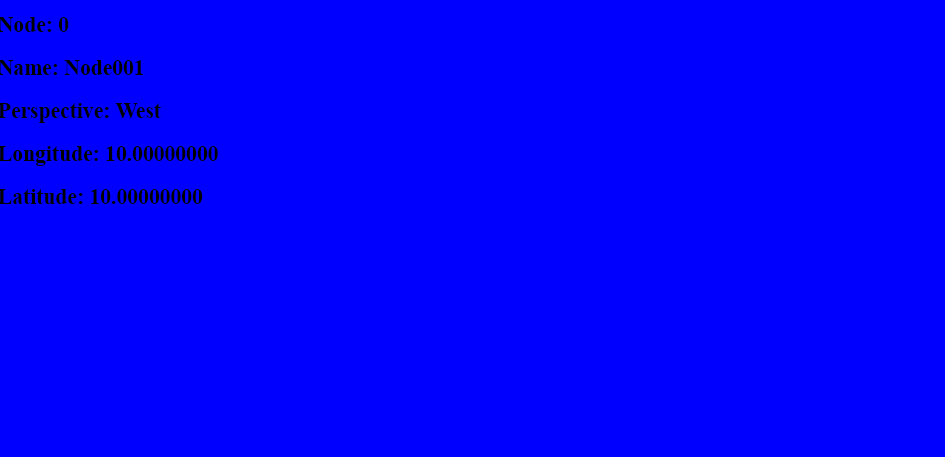
\includegraphics[width = \textwidth]{design/ui/profile}
        \caption{Node Profile}
        \label{fig:}
    \end{subfigure}%
    \begin{subfigure}[b]{0.5\linewidth}
        \centering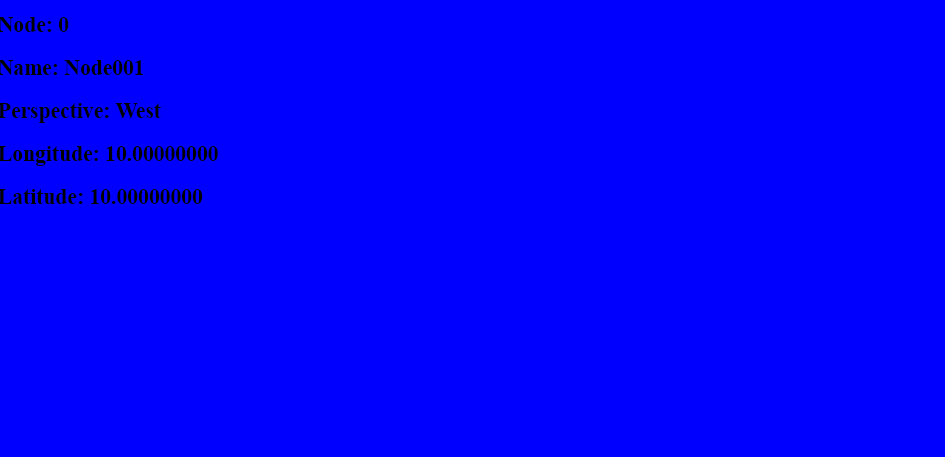
\includegraphics[width = \textwidth]{design/ui/profile}
        \caption{Live Video Feed}
        \label{fig:}
    \end{subfigure}
    \begin{subfigure}[b]{0.5\linewidth}
        \centering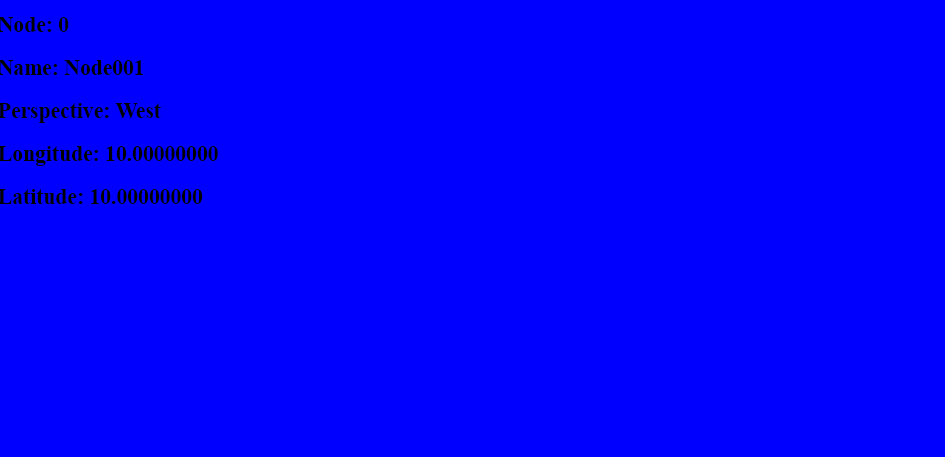
\includegraphics[width = \textwidth]{design/ui/profile}
        \caption{Vehicle Volume Plot}
        \label{fig:}
    \end{subfigure}
    \begin{subfigure}[b]{0.5\linewidth}
        \centering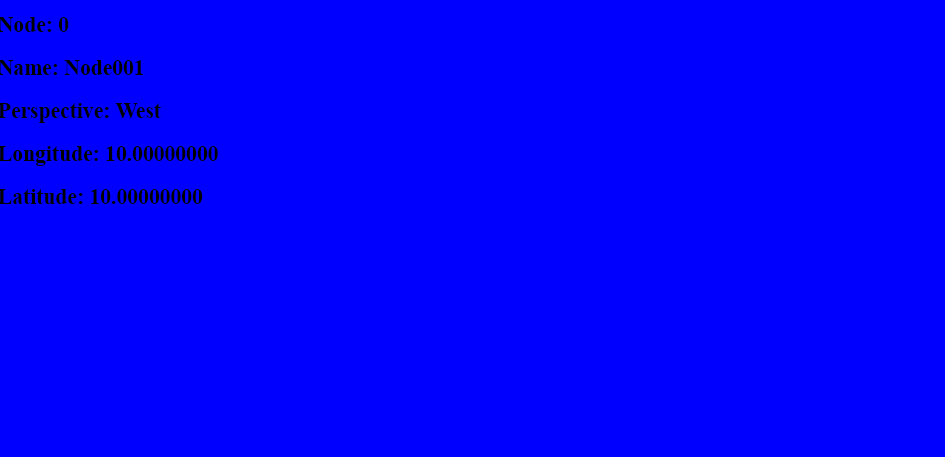
\includegraphics[width = \textwidth]{design/ui/profile}
        \caption{Vehicle Speed Plot}
        \label{fig:}
    \end{subfigure}
    \begin{subfigure}[b]{0.5\linewidth}
        \centering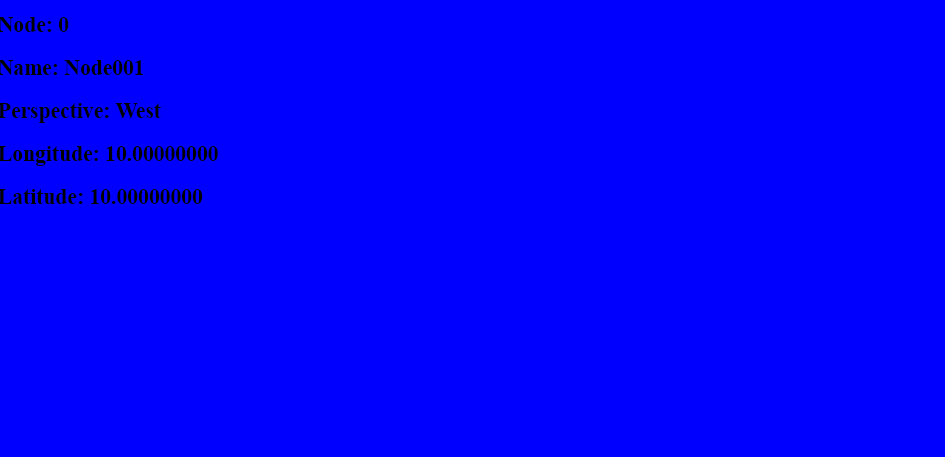
\includegraphics[width = \textwidth]{design/ui/profile}
        \caption{Whole Page View}
            \label{fig:}
    \end{subfigure}
    	\caption{Web Application - User Interface Panes}
    	\label{fig:dragonfly}
\end{figure}


